\chapter{Analysis of Bitcoin Price using Deep Learning Models}
Building on the work by Abraham on Cryptocurrency Price Prediction Using Tweet Volumes and Sentiment Analysis \cite{Abraham2018}, we gathered data from Twitter, Google Trends and Yahoo Finance about Bitcoin. That is, Tweets and Tweet Volume from Twitter, Search Value Index (SVI) from Google Trend, and Open, High, Low and Close value of Bitcoin hourly. We first explore the raw data gathered for any observable trend. Then, we perform feature engineering by cleaning the data, generating sentiment scores of Tweets using the state-of-art model roBERTa, identifying potential influencers using K-Means clustering, performing hourly aggregations and finally scaling the data. We then modelled the resulting dataset in two different ways. We used an LSTM NN model to predict the Bitcoin closing prices for the next 24hr.

\section{Data Collection}
In order to tackle the problem of prediction of Bitcoin prices, we gathered a large amount of data from different sources, which we believe might contribute information to predict the price. We first consider the sentiment analysis of Tweets from Twitter as our first input. We then get Bitcoin's Search Value Index (SVI) from Google Trends. Finally, we retrieved Bitcoin market prices from Yahoo Finance. All data are scrapped between 01 June 2022 and ending 13 July 2022.
\subsection*{Twitter}
In order to get Tweets related to Bitcoin from Twitter, we leverage Tweepy - an open-source Python Library for accessing the Twitter API. The API has different access levels: Essential, Elevated and Academic Research. We requested Academic Research access through the Twitter Developers Portal to get the appropriate API key and API token. Once access was provided, we used the query features from the documentation to scrape Tweets with either the word “bitcoin” or hashtag bitcoin (\#bitcoin). For each query, we collected the following information: username, user description, location, friends count, followers count, total tweets count, retweet count, hashtags in the tweets and the tweet.
\begin{lstlisting}[language=Python, caption= {Tweepy query for bitcoin, \#bitcoin and excluding re\-tweets}, label = tweet_search]
    query = 'bitcoin OR #bitcoin  lang:en -is:retweet'
\end{lstlisting}
The request cap for academic access is 100 per 15 minutes. We set up our scrapping strategy for 10 consecutive days at a rate of 65 Tweets a minute to match the request cap. This strategy allowed us to scrap 814,818 tweets with the query mentioned above. Additionally, we used the same access to get the tweet volume pertaining to the query in listing \refeq{tweet_search} and predefined start time and end time.

\begin{lstlisting}[language=Python, caption= {Tweepy query to get tweet count withing each hour between predefined start time and end time}, label= tweet_count]
    query_params = {'query': query ,'granularity': 'hour', 'start_time': start_time, 'end_time': end_time}
\end{lstlisting}
\subsection*{Google Trends}
Google is a massive search engine dealing with a vast amount of data daily, including the volume of searches of people based on keywords. Google trend data is a reflection of the volume of searches that people do. However, the data is extensive to be consumed directly due to the number of global users. The trend data is anonymised (personally identifiable information removed), categorised (topic associated with each search query) and aggregated (grouped). The trend data provided by Google are indexed to 100, where 100 is the maximum search interest for the time and location selected. The combination of the pre-processing of raw volume searches provides a measure of interest in a particular topic across different regions or globally.
We used the pytrends package - an unofficial open-source Python Library for accessing the Google trend data. We pass the least ambiguous keyword, “bitcoin”, into the library and retrieve the hourly search index for the said keyword.

\begin{lstlisting}[language=Python, caption= {pytrend query to get google trend index withing each hour between predefined start time and end time}, label = pytrend_search]
kw_list = ['bitcoin']
search_df = pytrends.get_historical_interest(kw_list, year_start=2022,month_start=6, day_start=1, hour_start=0, year_end=2022,month_end=7, day_end=16, hour_end=0,cat=0, geo='', gprop='')
\end{lstlisting}

\subsection*{Yahoo Finance}
In order to get Bitcoin prices, we used the yfinance package - an unofficial open-source Python Library for accessing market data on cryptocurrencies, regular currencies, stocks and bonds, fundamental and options data, and market analysis and news. We used the yfinance package to scrape the open, high, low and close prices and the volume of bitcoin traded hourly.
\begin{lstlisting}[language=Python, caption= {yfinance query to get bitcoin price and traded volume within each hour between predefined start time and end time}, label = yfinance_search]
BTC_Ticker = yf.Ticker("BTC-USD")
BTC_Data_long = BTC_Ticker.history(start="2022-06-01", end="2022-07-16",interval= '1h')
\end{lstlisting}
\par We briefly explore the raw data scrapped from the different sources to get a better understanding of the latter. The tweets from Twitter had several issues. A large number contained URLs, symbols, excessive punctuations and were in different languages (even if the query was restricted to English tweets only).
\begin{figure}[H]
    \centering
    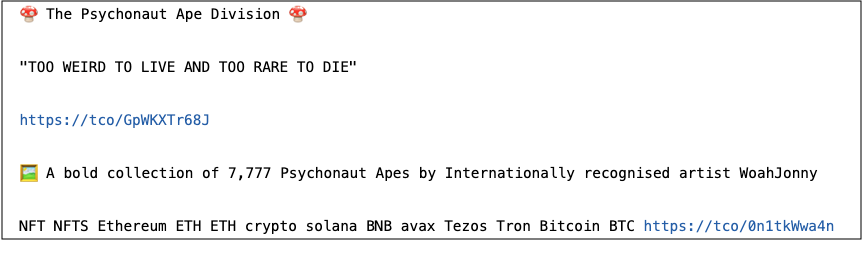
\includegraphics[scale=0.48]{CHAPTER_5/raw_tweet_example.png}
    \caption{Example of raw tweet scraped using the tweepy package through Python}
    \label{raw_tweet_example}
  \end{figure}
\noindent The number of tweets at the end of each hour was continuous and had no major issues from the API response.
\begin{figure}[H]
   \centering
   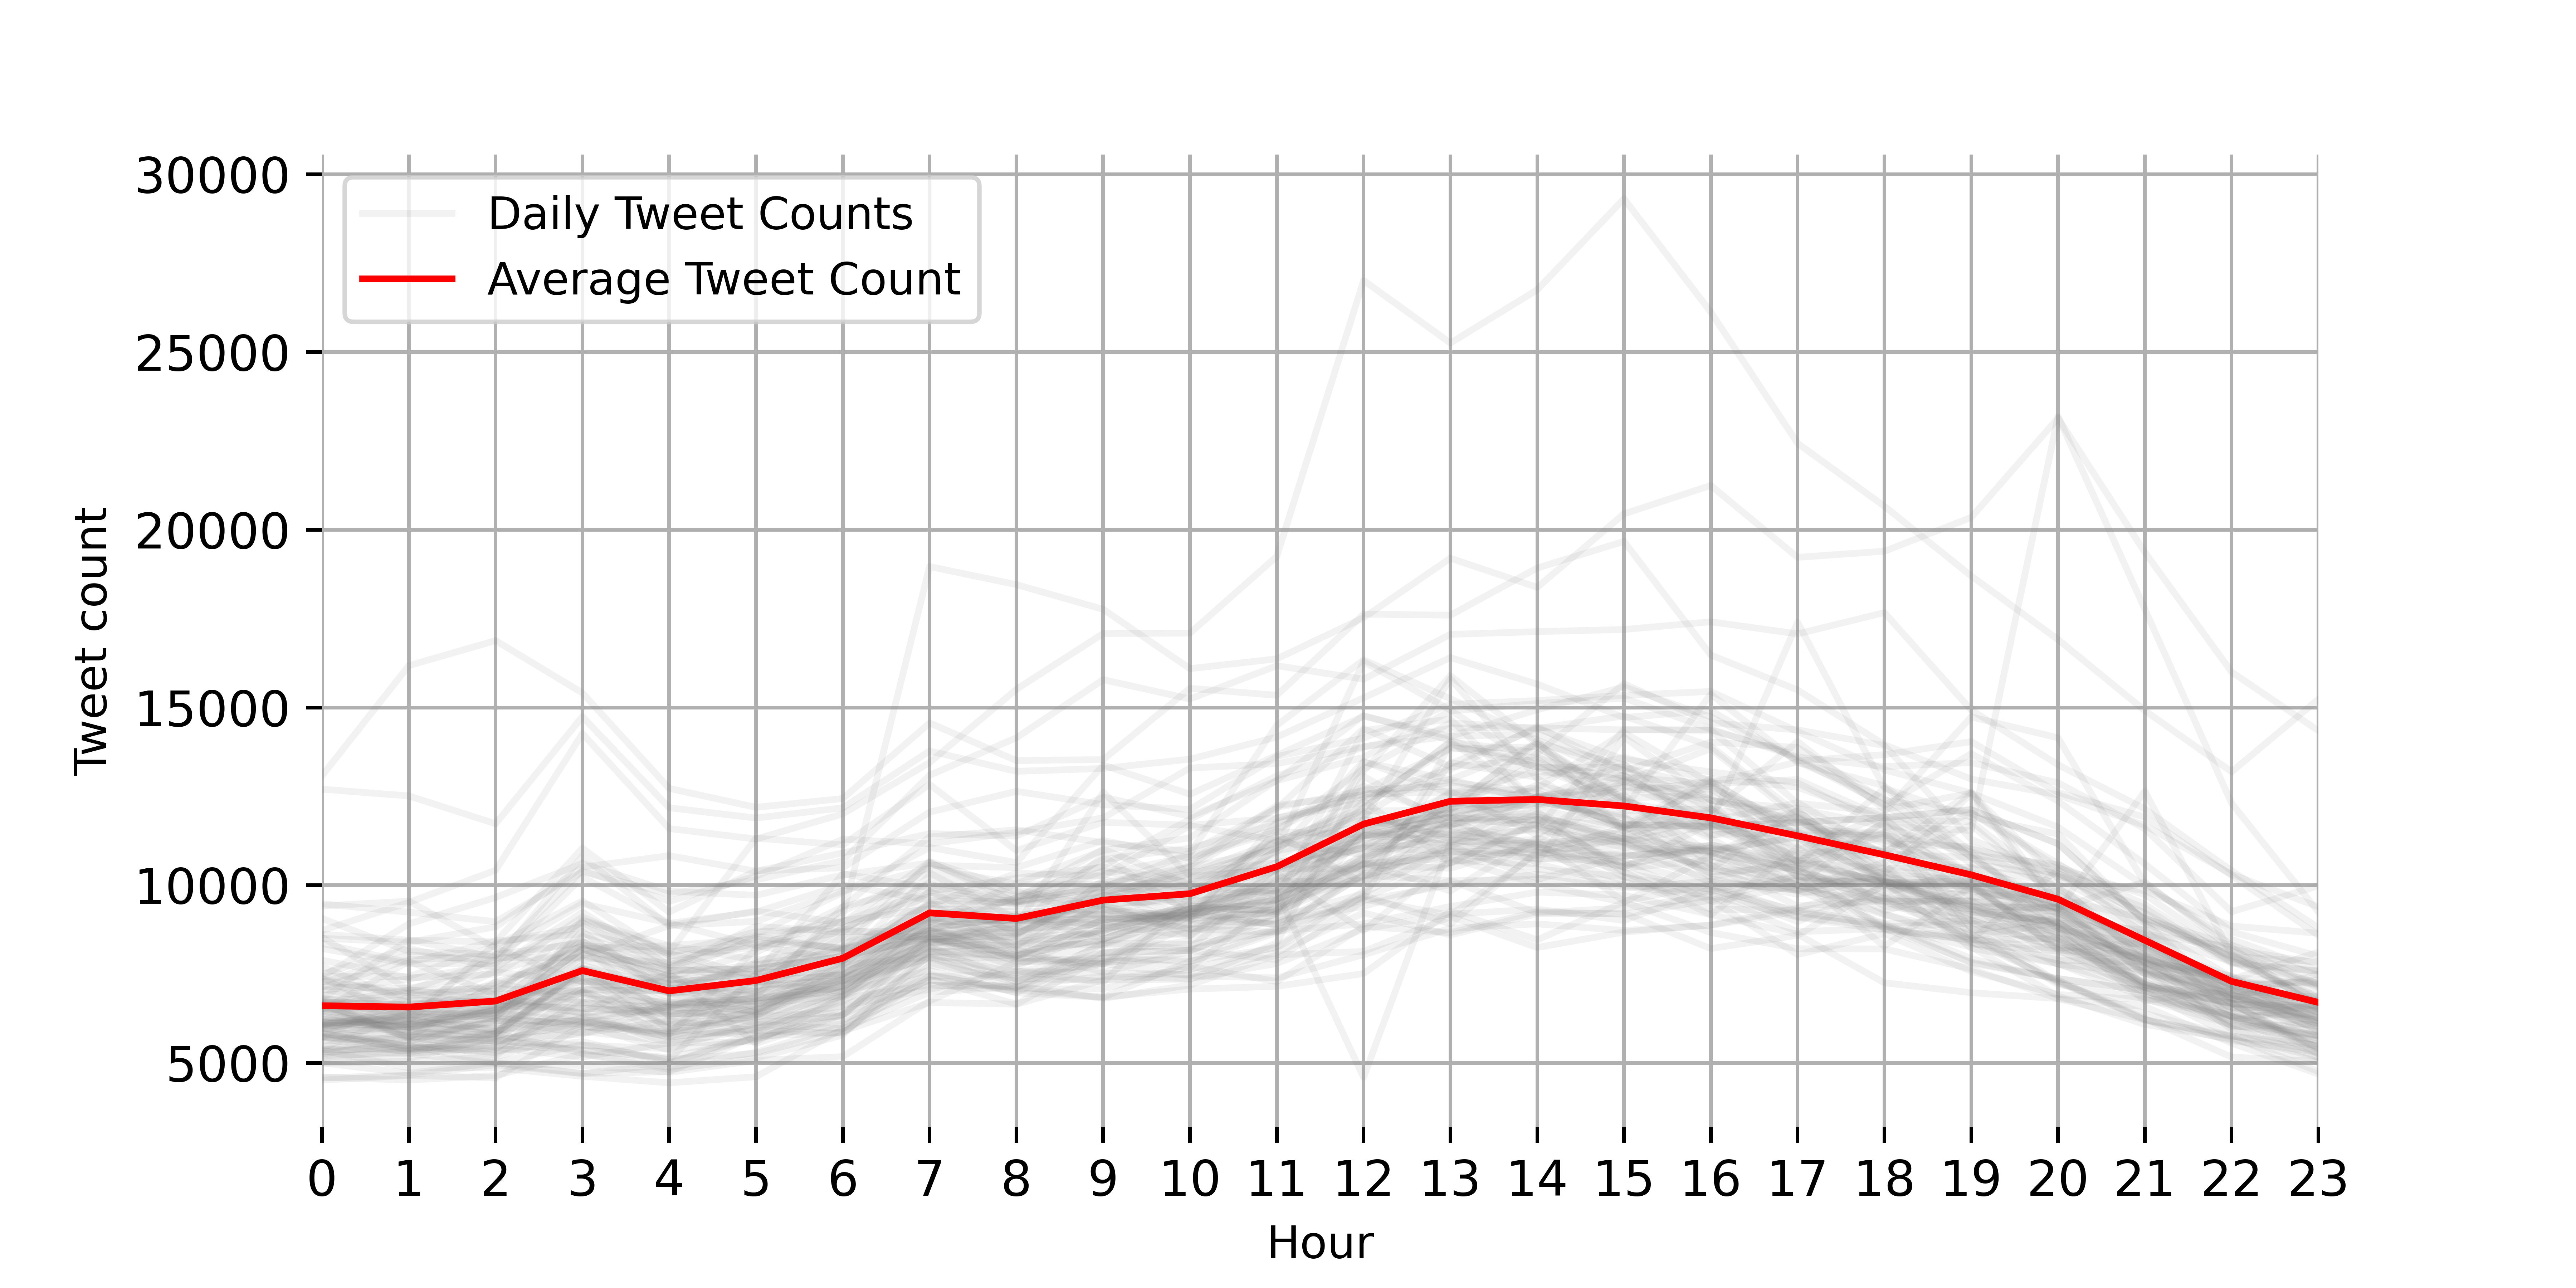
\includegraphics[scale=0.70]{CHAPTER_5/tweet_count_python.png}
   \caption{Distribution of tweet count over each day at the end of every hour over 24 hours}
   \label{tweet_count}
\end{figure}
\noindent The data for the open, high, low, and close prices scrapped from Yahoo Finance was clean and had no issues. However, we did see that not all closing hours have the associated volume. Thus, volume was not included in the final dataset.
\begin{figure}[H]
    \centering
    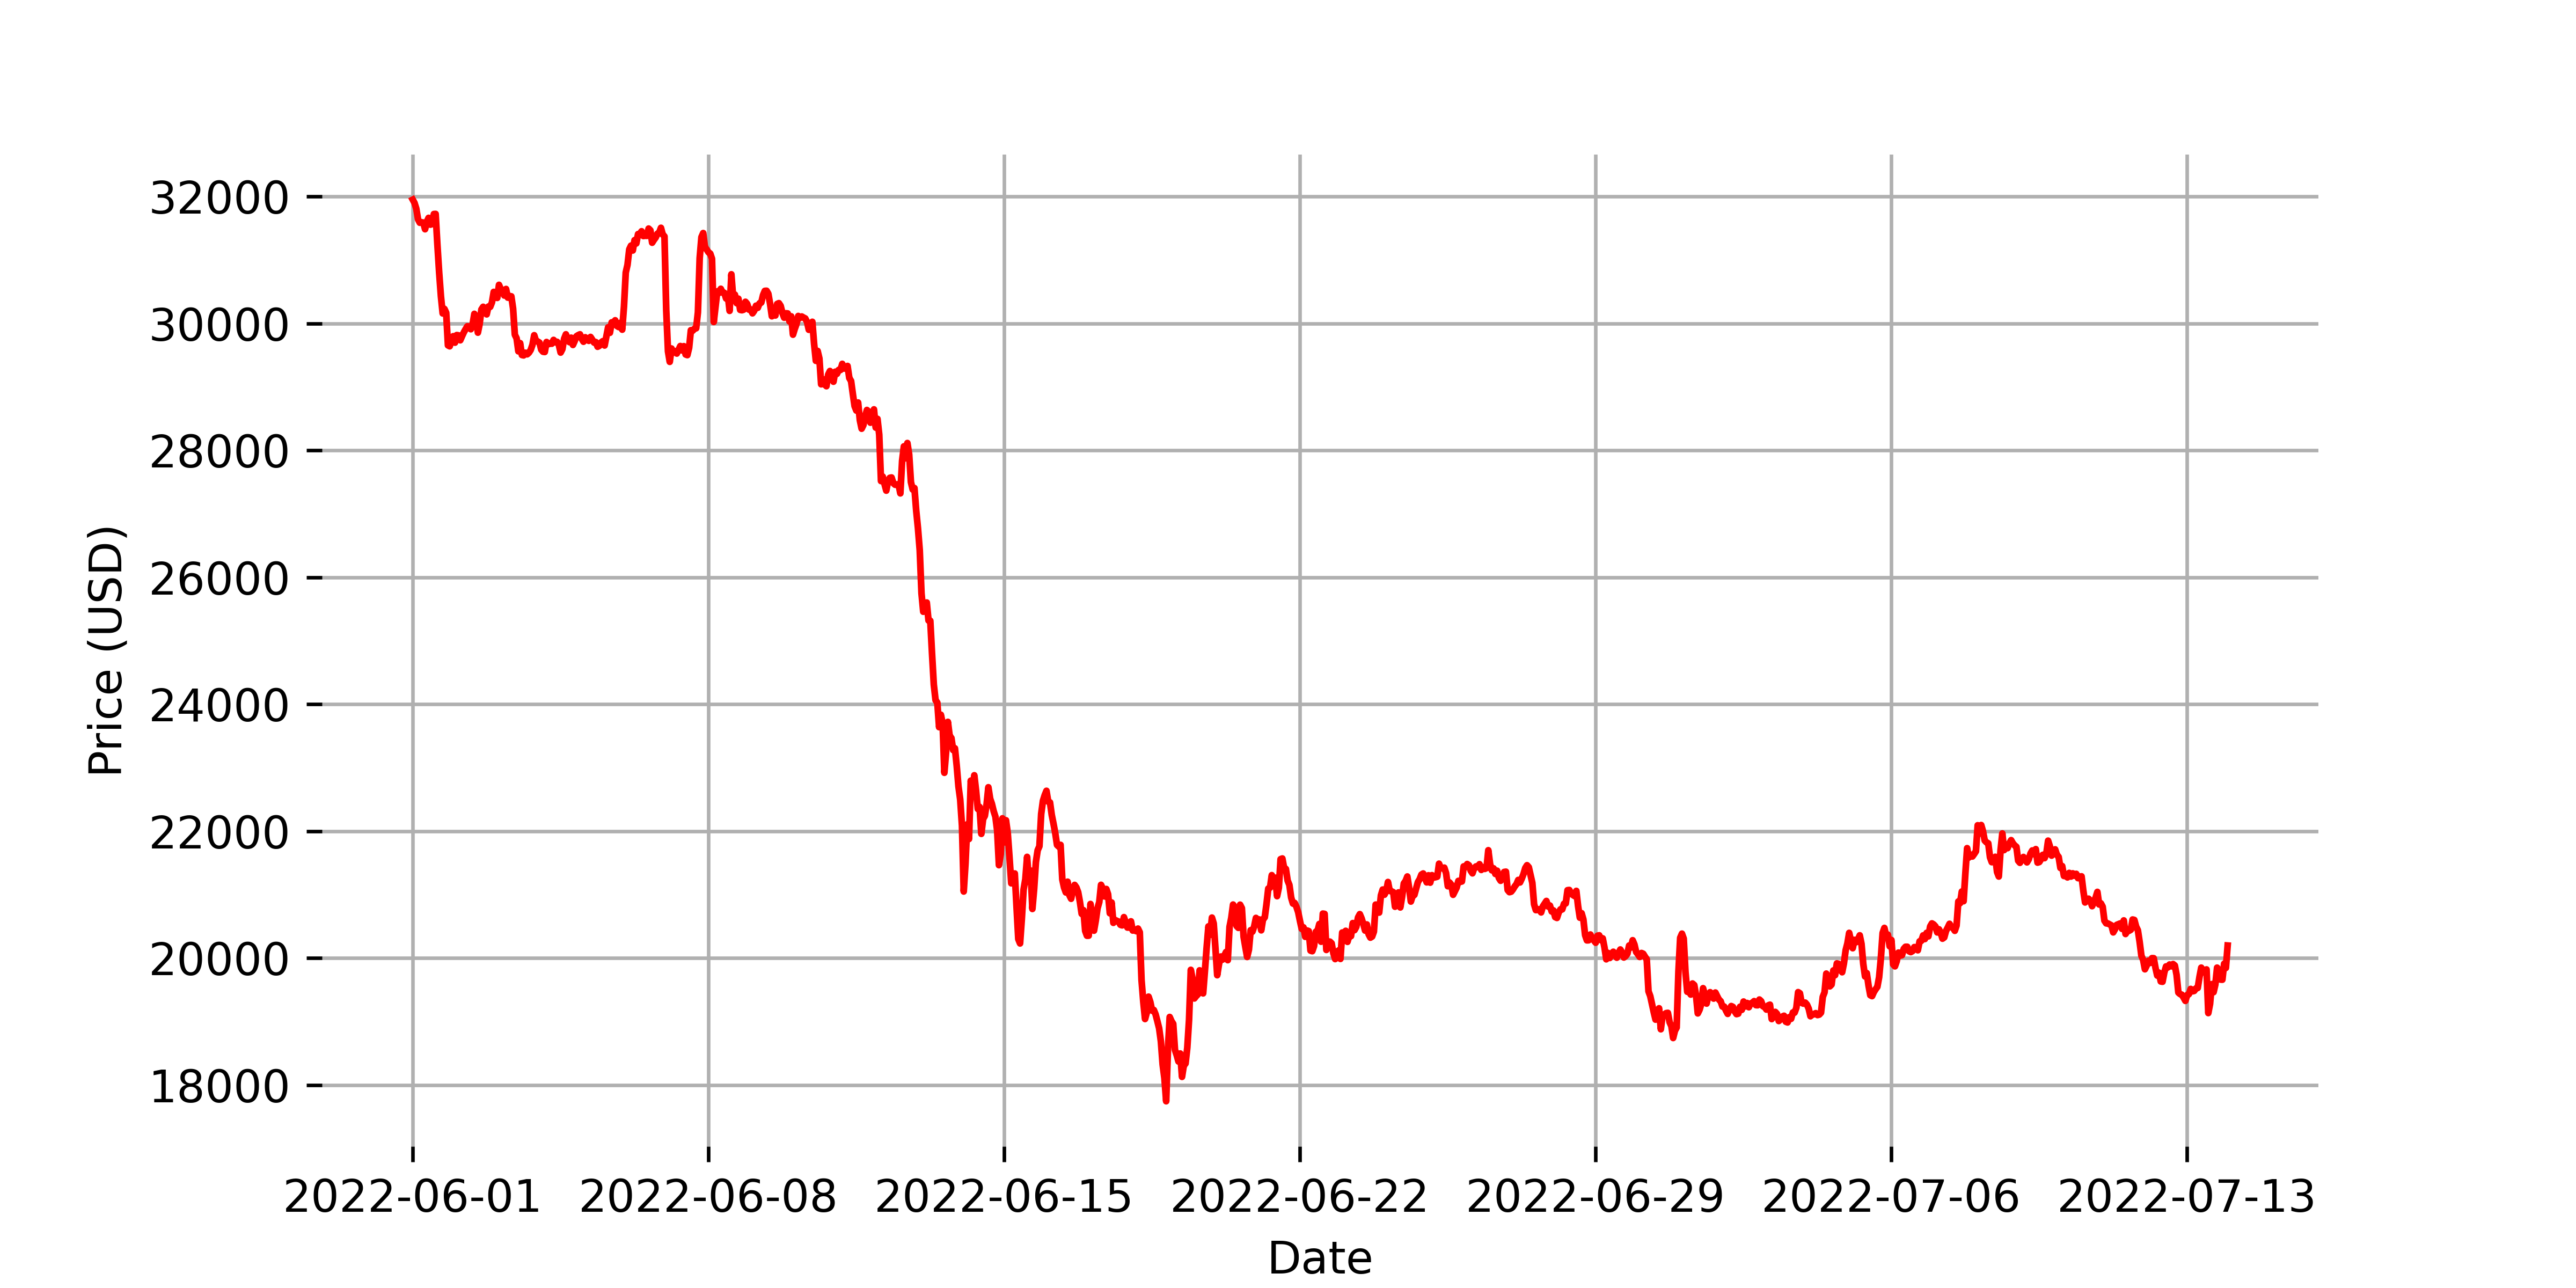
\includegraphics[scale=0.73]{CHAPTER_5/bitcoin_price_python.png}
    \caption{Bitcoin closing price over every hour for everyday}
    \label{bitcoin_price}
 \end{figure}
\section{Feature Engineering}
Feature engineering is the manipulation of our dataset to provide extra features to input in our model to improve accuracy. Manipulation includes addition, deletion, combination and transformation of the dataset. Practical feature engineering is dependent on the business problem and our objective. Common types of feature engineering include scaling and transformation, fitting missing values, feature coding, feature construction and feature extraction. 
\subsection*{Sentiment Analysis on Tweet Data}
In order to be able to quantify the tweets as features in our model, we transform the tweets into numerical values by performing sentiment analysis on them. However, as seen in the tweet example in listing (\ref{raw_tweet_example}), the raw tweet would be difficult for the existing natural language processing model to transform them. Using regular expression syntax in Python, we cleaned the tweets first.
\begin{lstlisting}[language=Python, caption= {Python function to clean Tweets using RegEx (regular expression)}, label= regex_function]
    def pre_process_tweet (text):
    #Remove all links starting with http...
    text = re.sub('https?:\/\/.*[\r\n]*','',text)
    #Remove RT
    text = re.sub('^RT[\s]+','',text)
    #Remove @[User]
    text = re.sub('@[^ ]+', '', text)
    #Remove Punctuation first
    text = text.translate(str.maketrans('','', string.punctuation))
    #Convert text to lower case
    text = text.lower()
    #Remove new line
    text = re.sub('\n',' ',text)
    #Replace emojis with description
    text = demoji.replace_with_desc(text,sep=' ')
    #Reducing whitespaces to one everywhere
    text = re.sub('\s+',' ',text)
    return text
\end{lstlisting}
Applying the python function defined in listing \ref{regex_function} to the raw tweet in \ref{raw_tweet_example} leads to the following string:
\begin{align}
    \label{preprocess_tweet}
    \nonumber
    &\text{'mushroom the psychonaut ape division mushroom too weird to live and too } \\
    \nonumber
    &\text{rare to die framed picture a bold collection of psychonaut apes by  }\\
    \nonumber
    &\text{internationally recognised artist woahjonny nft nfts ethereum eth eth crypto }\\
    &\text{solana bnb avax tezos tron bitcoin btc'}
\end{align}
We apply the pre-process tweet function across the 814,818 tweets that were scraped. Thus, making the tweets easier to process in sentiment analysis models. Once the tweets are clean, we use the RoBERTa model defined in Section \ref{section: transformers} to perform sentiment analysis. We used the version \textit{cardiffnlp/twitter-roberta-base-sentiment} which is made available Hugging Face. 'Twitter-roBERTa-base' for Sentiment Analysis is a pretrained  on approximately 58 million tweets and fine-tuned for sentiment analysis \cite{France2020}. The output of the model are is the percentage of a tweet being negative, neural and positive.
\begin{lstlisting}[language=Python, caption= {Applying the twitter-roberta-base-sentiment model to the preprocessed tweet in (\ref{preprocess_tweet})}, label= roberta_example]
    encoded_text = tokenizer(preprocessed_tweet, return_tensors='pt')
    output = model(**encoded_text)
    scores = output[0][0].detach().numpy()
    scores = softmax(scores)
    scores_dict = {'roberta_neg':scores[0], 'roberta_neu':scores[1], 'roberta_pos':scores[2]}
    print(scores_dict)

>> {'roberta_neg':0.298603, 'roberta_neu':0.5974009, 'roberta_pos':0.10399604}
\end{lstlisting}
We apply the same function through the whole preprocessed dataset to get the scraped tweets' scores. Tweets that were too long or had unknown characters that the model could not process were dropped (less than 0.5\% of the tweet dataset). 
\begin{figure}[H]
    \centering
    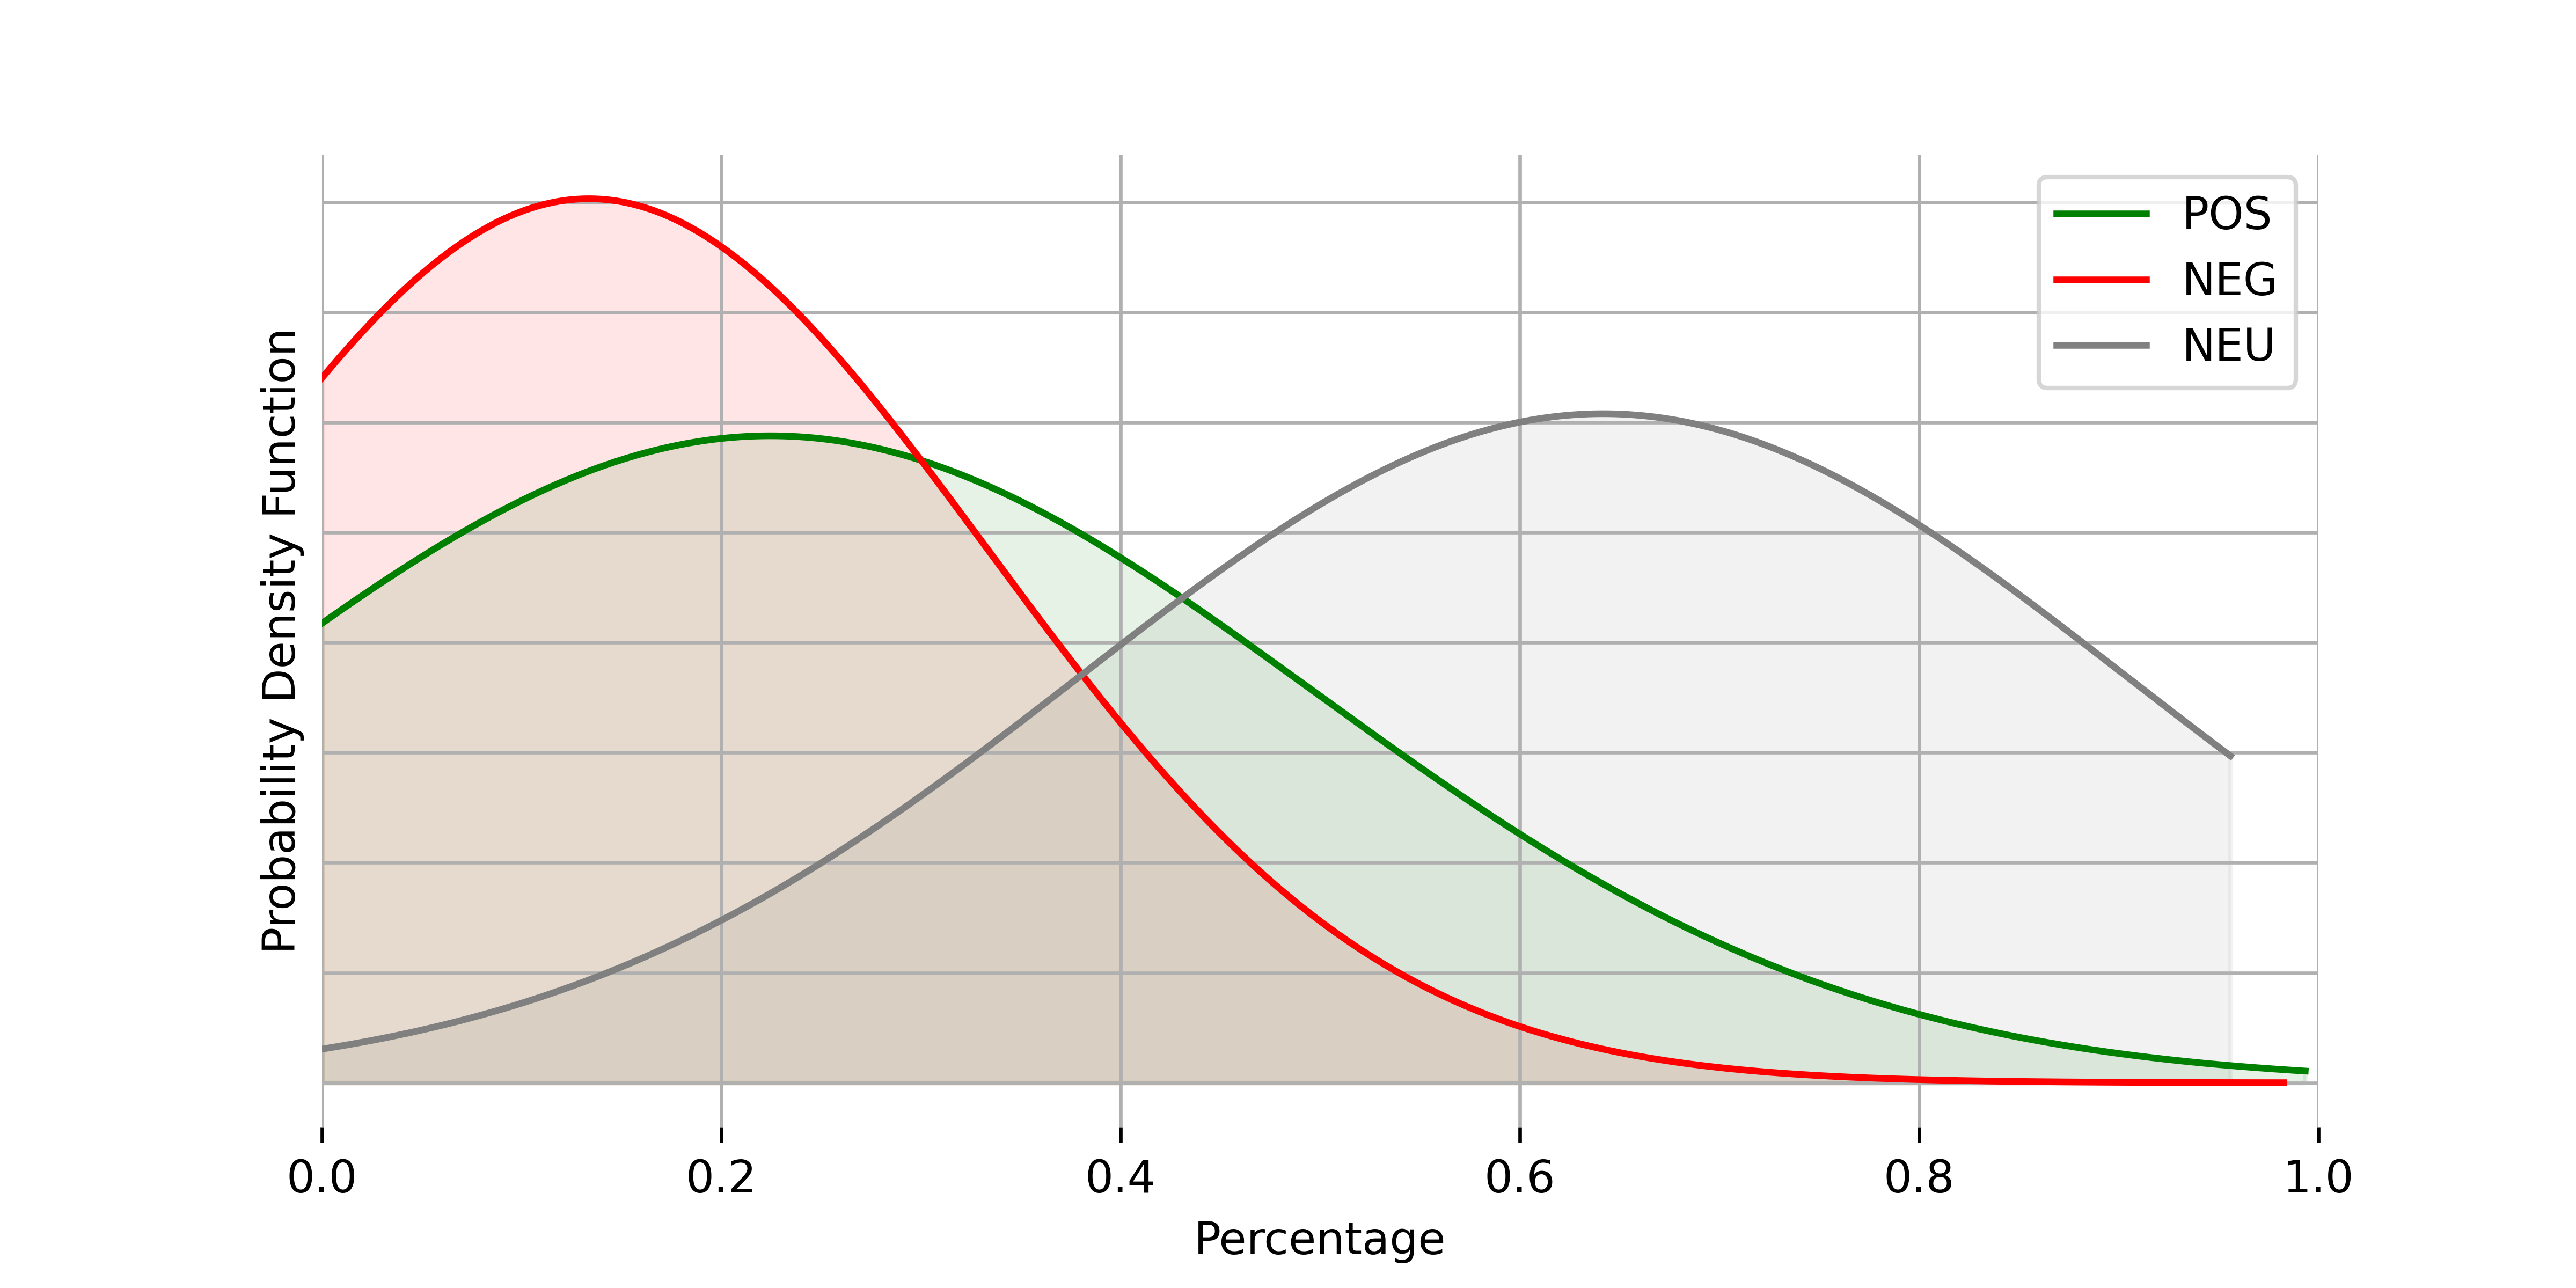
\includegraphics[scale=0.6]{CHAPTER_5/sentiment_score_distribution_python.png}
    \caption{Sentiment score distribution using roBERTa model on all tweets}
    \label{sentiment_score_distribution}
 \end{figure}
\subsection*{Data Encoding}
Data encoding involves choosing a set of symbolic values to represent different categories. The symbolic values can take input a single or multiple columns and produce a category on top of the dataset. For example, indicating whether the collected data on a holiday can be coded as 1 and 0 otherwise. In our case, we attempt to separate the influencers from ordinary people by studying the total number of followers of the user that tweeted about Bitcoin. Using KMeans clustering, we group users based on their number of followers. We then excluded users within the group with the least number of followers to get only "influencer" users.
\begin{figure}[H]
    \centering
    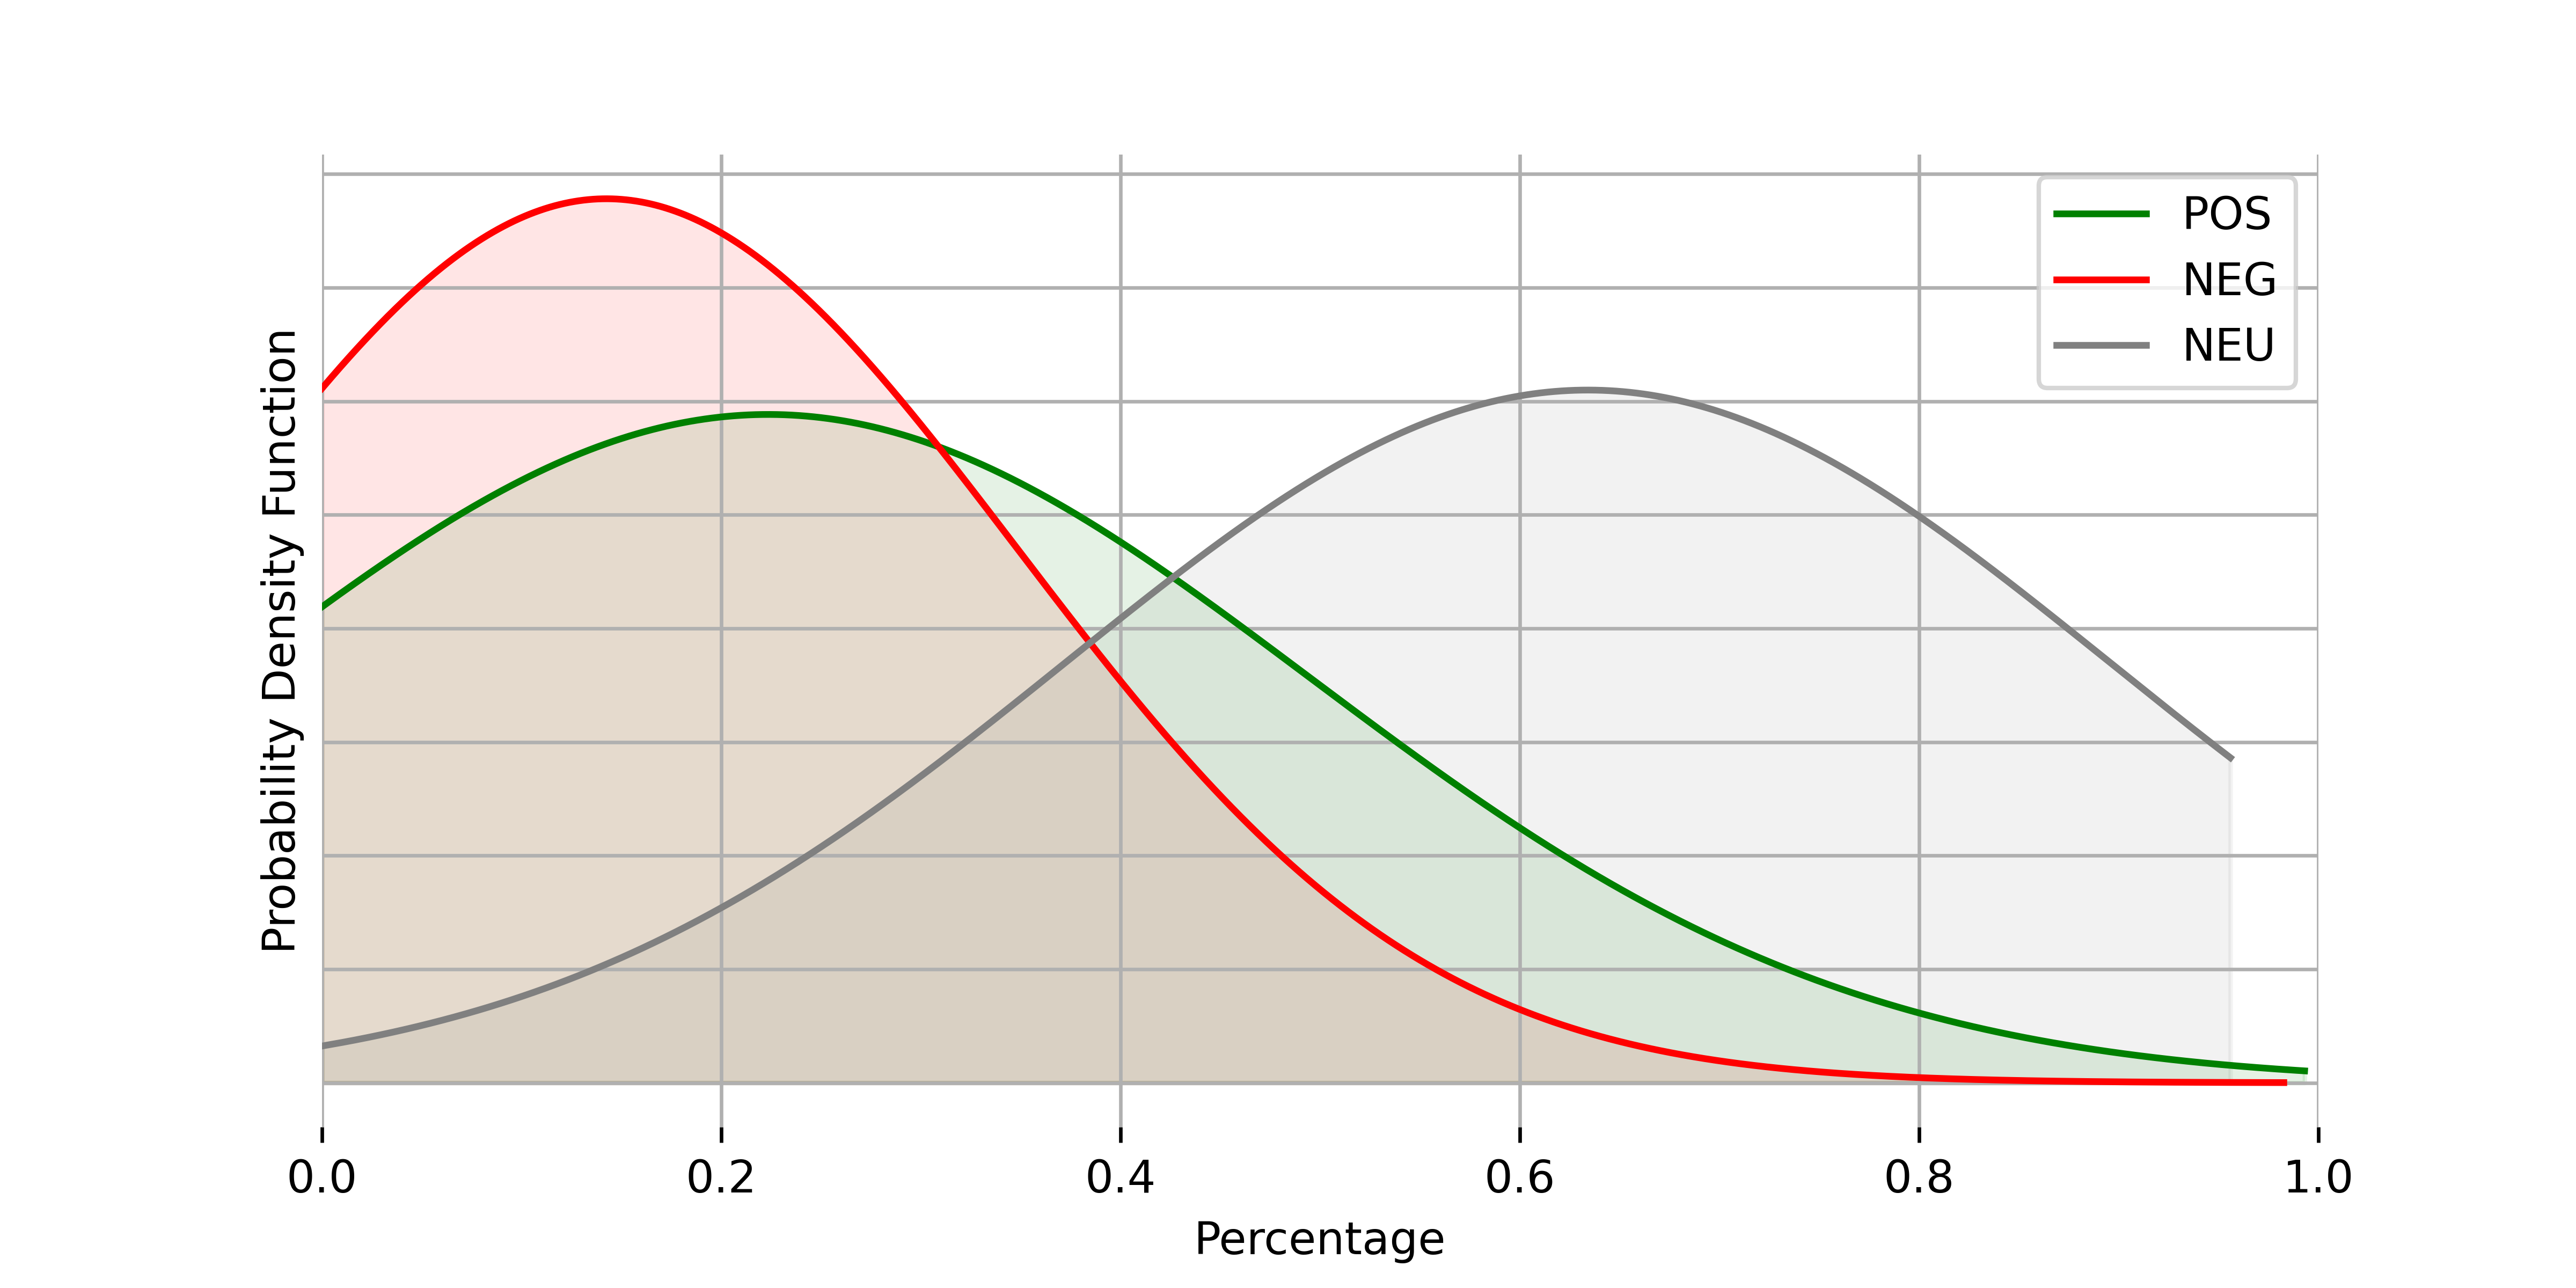
\includegraphics[scale=0.6]{CHAPTER_5/sentiment_score_distribution_python_inf.png}
    \caption{Sentiment score distribution of Twitter influencers (grouped using KMeans clustering) using roBERTa model on all tweets}
    \label{sentiment_score_distribution_influencers}
 \end{figure}
\subsection*{Scaling}
Scaling refers to the adjustment of large dataset to ease the learning process and also prevent large values to dominate when building a predictive model.
Processing the point data of all the scrapped tweets can be overly demanding in terms of computational power. This may result to an overfitting and not being able to model the general trend of a single day. Additionally, we do not have point data for price and google trends search index. To overcome this problem, we aggregated the sentiment scores (POS, NEU, NEG) over each hour across the time period. The resulting dataset was $1032 \times 3$ (24 hourly intervals for 43 days).
Moreover, our dataset consists of various data sources with overly different means. In order to prevent any feature to dominate the dataset, we scaled our features using the min/max feature scaling so that our values fall between -1 and 1 for all features.
\begin{figure}[H]
    \centering
    \includegraphics[scale=0.85]{CHAPTER_5/feature_engineering_pipeline.png}
    \caption{Feature engineering pipeline}
    \label{feature_eng_pipeline}
 \end{figure}
\section{Modelling Bitcoin Price using LSTM NN}
In order to predict the price of Bitcoin for the next 24 hours based on the information from the past day, we need to use sequential models. We used a Long-Short-Term-Memory neural network model for prediction because of its ability to retain long- and short-term information. Using the feedback loop in the architecture, we can model dependencies within the data, and the hidden cell allows for a generalisation of the data for the window (24 hours in our case). We used the scaled preprocessed from the previous section with a rolling forecast of 1 day (24 hours) to predict the next day (24 hours). The training dataset contained 41 days (42, if the rolling window is included). The latter comprises 6 features from each hour: tweet volume, Google trend search index, average tweet sentiment (positive, negative, neutral), and price of Bitcoin, and the label (target) was the price of Bitcoin in the next hour.


\begin{figure}[H]
   \centering
   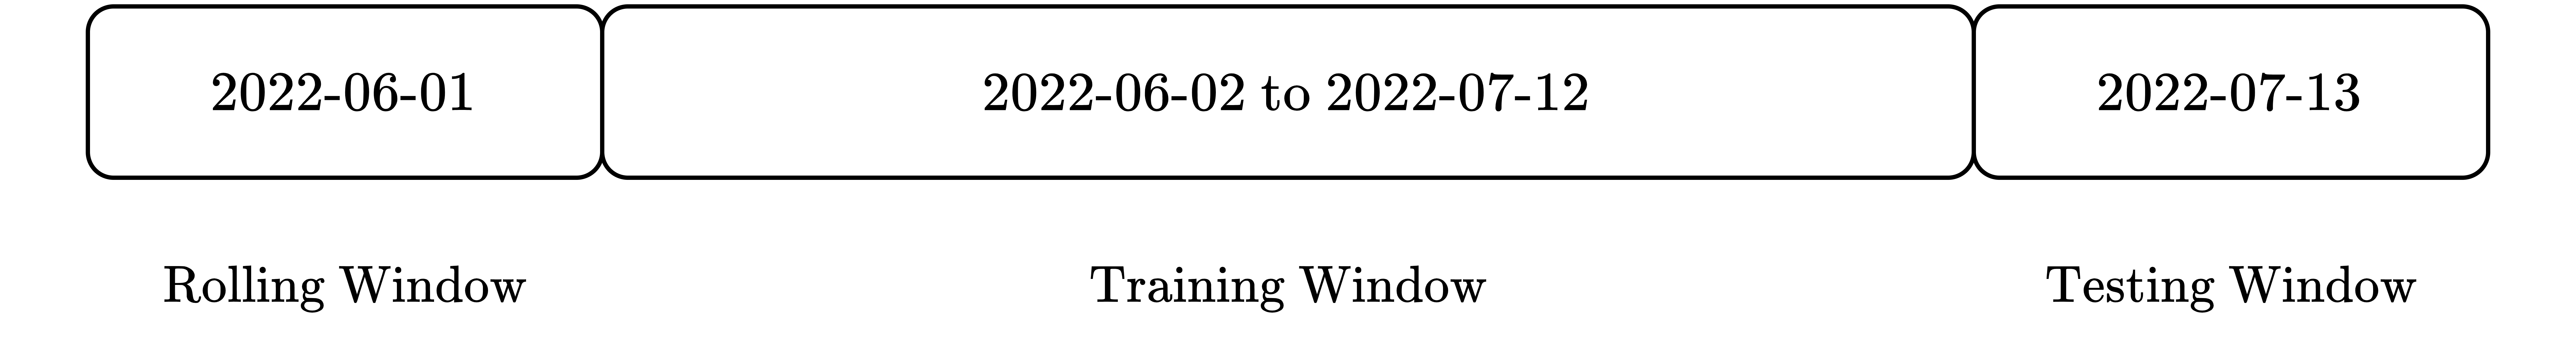
\includegraphics[scale=0.90]{CHAPTER_5/train_test_split.png}
   \caption{Train-test split}
   \label{train_test_split}
\end{figure}


 \noindent After experimentation, we found that using an LSTM NN with 50 hidden states, 250 epochs and a learning rate $\alpha = 0.00001$ converges. The loss was calculated using the mean squared error within the network. We used the Adam optimizer to train the network faster.

 \begin{figure}[H]
    \centering
    \includegraphics[scale=0.9]{CHAPTER_5/LSTM_architechture.png}
    \caption{LSTM architecture with 50 hidden states, input sequence of 25 and 6 input features}
    \label{LSTM_architechture}
 \end{figure}
\section{Results}
The training is set to run for 250 epochs which took around 1 hour to complete. We observed that the MSE in the model training was down to 0.0146 (ADD REF FIGURE). However, it is not interpretable since the data was scaled when processed in the model. The training at each epoch is extracted and the inverse transform is performed. We then computed the RMSE (for interpretability) for the training and observed that it was \$303.96 after 250 epochs. The testing error for the next 24 hours was \$325.96.  
\begin{figure}[H]
   \centering
   \includegraphics[scale=0.55]{CHAPTER_5/LOSS_MODEL_MSE.png}
   \caption{Model training loss (MSE) and actual training loss in USD (RMSE) over 250 epochs of training}
   \label{training_loss}
\end{figure}
\noindent We also noticed that after only 25 epochs, the general profile of the Bitcoin price is replicated by the model.
 \begin{figure}[H]
    \centering
    \includegraphics[scale=0.42]{CHAPTER_5/epoch_graph.png}
    \caption{Model evolution during training for epochs 1, 5, 25 and 250}
    \label{epoch_graph}
 \end{figure}
\noindent After training for 250 epochs, we used the model to calculate a rolling window forecast on the price for the next 24 hours. We observe that the general profile of the price movement is modelled but sudden dips and rise in price were not replicated during testing.
\begin{figure}[H]
   \centering
   \includegraphics[scale=0.55]{CHAPTER_5/result_pred.png}
   \caption{Trained model and rolling window forecast for Bitcoin price for next 24 hours (using whole dataset)}
   \label{result_pred}
\end{figure}
\noindent We ran a different experiment with the limited dataset containing only influencers but did not observe any major improvement from the previous experiment. On the contrary, we noticed a slight increase in RMSE in training and testing. \vspace{5mm}

\begin{figure}[H]
   \centering
   \includegraphics[scale=0.40]{CHAPTER_5/result_pred_inf.png}
   \caption{Trained model and rolling window forecast for Bitcoin price for next 24 hours (using influencers' dataset)}
   \label{result_pred_inf}
\end{figure}
\begin{table}[H]
    \begin{center}
        \begin{tabular}{l |c |c }
        \label{result_summary}
            
              & Experiment 1 & Experiment 2\\ &Complete Dataset & Influencers' Dataset\\
            \hline
            Model Training MSE & 0.0146 & 0.0209 \\
            
            Actual Training RMSE & \$303.96 & \$317.45\\
            Actual Testing RMSE & \$325.96 & \$335.99\\

        \end{tabular}
        \caption{Summary of error results from model using the complete dataset and the influencers' dataset using the same training and prediction scenario.}
    \end{center}
\end{table}\vspace{5mm}

    
%\section{Modelling Bitcoin Upticks using Feedforward NN}
%\subsection*{Model Architecture and Hyperparameters}
%No Influencer
%With Influencer
%Comparison